\chapter{Introduction to the \textsc{promethee} methods}
\label{chapterPromethee}

The \textsc{promethee} (Preference Ranking Organisation METHod for Enrichment Evaluations) methods are outranking methods that have been developed at the \textsc{Universit\'{e} Libre de Bruxelles} and the \textsc{Vrije Universiteit Brussel} since the beginning of the 80'.
Initially proposed by J.P. Brans in 1982,  %maybe make citation
they are used to address multi-criteria problems.

The \textsc{promethee} family is relatively young compared to some other multi-criteria decision aid methods but have experienced a rapid spread as it can be seen from the increasing amount of papers that are written each year about them \cite{Behzadian2010198}.

The \textsc{promethee} methods must be applied on problems with a finite set of alternatives and a finite family of criteria.
The information about each alternative and its evaluations for each criterion can be summarized in a table such as Table \ref{tbl:evaluation_table}.

\begin{table}[h]
\center
\begin{tabular}{ L @{\hskip 1cm}L L L L L}
    \toprule
    a        & f_1(.)               & \dots  & f_c(.)        & \dots  & f_k(.) \\ [7pt]
    \midrule
    a_1      & f_1(a_1)             & \dots  & f_c(a_1)      & \dots  & f_k(a_1)\\
    \vdots   & \vdots               & \ddots & \vdots        & \ddots & \vdots \\
    a_i      & f_1(a_i)         & \dots  & f_c(a_i)  & \dots  & f_k(a_i)  \\
    \vdots   & \vdots               & \ddots & \vdots        & \ddots & \vdots \\
    a_n      & f_1(a_n)             & \dots  & f_c(a_n)      & \dots  & f_k(a_n)\\
    \bottomrule
\end{tabular}
\caption{example of evaluation table}
\label{tbl:evaluation_table}
\end{table}

\newpage

This raw information is generally not directly usable by the decision maker.
 \textsc{promethee} offer some tools to help him in his ordering, choice, sorting problem, etc.

These methods are based on the three followings concepts \cite{Bertrand2002}:
\begin{enumerate}
    \item \textbf{Enrichment of the preference structure } \\
        For each criterion, a preference function is introduced.
        These preference functions are aimed at indicating the degree at which one alternative is prefered over another for that specific criterion.
        This is done by taking into account the deviation's amplitude between the evaluations of the two alternatives regarding the concerned criterion.
        This leads to an enriched intra-criterion preference structure of the alternatives. \\
        This procedure also allows to get rid of all the scaling effects due to the measuring system used to express the different criteria.
    \item \textbf{Enrichment of the dominance relationship} \\
        For each couple of alternatives, a global preference index of the one over the other will be computed using the previously defined preference functions on all the criteria.
        Using these global preference indices, a quantitative outranking score is computed.
    \item \textbf{Decision support} \\
        An outranking relation is used to rank the alternatives according to their outranking scores. This relation is used to provide some insights to the decision maker.
\end{enumerate}

\section{Enrichment of the preference structure}
\label{sec:pref_struct}

First of all, let us introduce the notation $d_c(a_i,a_j)$ that will represent the difference between $f_c(a_i)$ and $f_c(a_j)$:
\begin{equation}
    d_c(a_i,a_j) = f_c(a_i) - f_c(a_j)
    \label{eq:dc}
\end{equation}

As pointed out by \cite{brans1994promcalc}, the natural dominance relation defined in section \ref{sec:multi_criteria_dominance_rel} is often very poor.
An alternative $a_i$ is dominating another alternative $a_j$ only if there is unanimity on all the criteria. This means that the evaluation for every criterion of the alternative $a_i$ must be at least as good as the evaluations on the corresponding criterion of $a_j$. This is generally not the case due to the conflicting nature of the criteria (for instance, a smartphone with a better battery will generally be heavier than one with a poor battery). \\
Furthermore only the signs of the differences between the evaluations are taken into account and not their amplitudes.
A difference of amplitude $d_c$ of $1\%$ between $f_c(a_i)$ and $f_c(a_j)$ should generally (but not always) not have the same impact as a difference of $200\%$ (see the rubber composition choosing problem on page \pageref{sec:drawback_monocriteria}).
% As pointed out by \cite{brans1994promcalc}, the natural dominance relation defined in section \ref{sec:multi_criteria_dominance_rel} has the following shortcomings:

% \begin{enumerate}
%     \item \textbf{the relation can be misleading:} \\
%         Only the sign of the difference between the evaluations is taken into account and not the amplitudes of these differences.
%         A difference of amplitude $d_c$ of $1\%$ between $f_c(a_i)$ and $f_c(a_j)$ should generally not have the same impact as a difference of $200\%$ (see the rubber composition choosing problem example on page \pageref{sec:drawback_monocriteria}).
%     \item \textbf{the relation is poor:} \\
%         An alternative $a_i$ is dominating another alternative $a_j$ only if there is unanimity on all the criteria. This means that the evaluation for every criterion of the alternative $a_i$ must be at least as good as the evaluations of the corresponding criterion of $a_j$. This is generally not the case due to the conflicting nature of the criteria (for instance, a smartphone with a better battery will generally be heavier than one with a poor battery).
% \end{enumerate}

To cope with this disadvantage, the preference structure will be enriched with the new notion of \textit{preference functions}. These preference functions $P_c(a_i,a_j)$ will give the preference degree of alternative $a_i$ over $a_j$ on the criterion $c$ in function of the difference $d_c$ between $f_c(a_i)$ and $f_c(a_j)$:

\begin{equation}
    P_c(a_i,a_j)  = P_c[d_c(a_i,a_j)]
    \label{eq:generalised_criterion}
\end{equation}

The preference degree will be between $0$ and $1$ and will be valued as follow \cite{Bertrand2002}:


\begin{equation}
    \left\{
    \renewcommand{\arraystretch}{1.75}
    \begin{array}{l c c c c c c}
        P_c(a_i, a_j) = 0       & if & d_c(a_i,a_j) & \le & 0 & \text{(no preference)} \\
        P_c(a_i, a_j) \approx 0 & if & d_c(a_i,a_j) & >   & 0 & \text{(weak preference)} \\
        P_c(a_i, a_j) \approx 1 & if & d_c(a_i,a_j) & > > & 0 & \text{(strong preference)} \\
        P_c(a_i, a_j) = 1       & if & d_c(a_i,a_j) & >>> & 0 & \text{(strict preference)} \\
    \end{array} \right .
    \label{eq:preference_function_values}
\end{equation}

To be compatible with the meaning of preference, the preference functions must be nondecreasing and must be equal to $0$ for any negative difference of evaluation ($d_c(a_i,a_j) \le 0$).

The decision of a preference function satisfying these conditions is let to the decision maker. However, a set of $6$ different types are proposed in \cite{Bertrand2002} which should satisfy the majority of them:

\subsubsection{Type 1: the usual criterion}
\begin{figure}[H]
\begin{minipage}{.5\textwidth}
    \begin{center}
    \begin{tikzpicture}
    \draw[->] (-1.5,0) -- (3,0);
    \draw (3,0) node[below=0.1cm] {$d_c$};
    \draw [->] (0,0) -- (0,3);
    \draw (0,3) node[left=0.1cm] {$P_c$};
    \draw (0,0) node[below=0.1cm] {$0$};
    \draw[dashed] (-1.5,2) -- (3,2);
    \draw[domain=-1.5:0.025,smooth,variable=\x,blue,line width=0.5mm] plot ({\x}, {0});
    \draw[domain=0:2.025,smooth,variable=\y,blue,line width=0.5mm] plot ({0}, {\y});
    \draw (0,2) node[above left=0.01cm] {$1$};
    \draw[domain=0:3,smooth,variable=\x,blue,line width=0.5mm] plot ({\x}, {2});
    \end{tikzpicture}
    \end{center}
\end{minipage}%
\begin{minipage}{.5\textwidth}
    \begin{equation}
        P_c = \left\{
            \begin{array}{l c c}
                0 & \text{if} & d_{c} \le 0 \\
                1 & \text{if} & 0 < d_c \\
            \end{array}
            \right .
        \label{eq:type1_criterion}
    \end{equation}
\end{minipage}
\caption{Preference function of the usual criterion}
\end{figure}

This criterion does not imply any extension of the classical notion of preferences. As soon as the evaluation between the two alternatives is not identical, there will be a strict preference for the alternative having the highest evaluation.
This criterion is therefore not enriching the preference structure but allows the decision maker to use the criteria in their usual sense, without having to define any parameter. 
This preference function is also useful when using the amplitude between two evaluations does not make sense. 

\subsubsection{Type 2: the quasi-criterion}
\begin{figure}[H]
\begin{minipage}{.5\textwidth}
    \begin{center}
    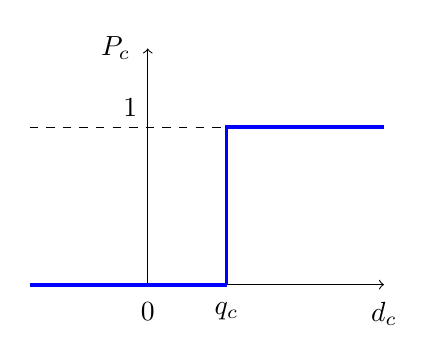
\begin{tikzpicture}
    \draw[->] (-1.5,0) -- (3,0);
    \draw (3,0) node[below=0.1cm] {$d_c$};
    \draw [->] (0,0) -- (0,3);
    \draw (0,3) node[left=0.1cm] {$P_c$};
    \draw (0,0) node[below=0.1cm] {$0$};
    \draw[dashed] (-1.5,2) -- (3,2);
    \draw[domain=-1.5:1,smooth,variable=\x,blue,line width=0.5mm] plot ({\x}, {0});
    \draw (1,0) node[below=0.1cm] {$q_c$};
    \draw[domain=0:2.025,smooth,variable=\y,blue,line width=0.5mm] plot ({1}, {\y});
    \draw (0,2) node[above left=0.01cm] {$1$};
    \draw[domain=1:3,smooth,variable=\x,blue,line width=0.5mm] plot ({\x}, {2});
    \end{tikzpicture}
    \end{center}
\end{minipage}%
\begin{minipage}{.5\textwidth}
    \begin{equation}
        P_c = \left\{
            \begin{array}{l c c}
                0 & \text{if} & d_{c} \le q_c \\
                1 & \text{if} & q_c < d_c \\
            \end{array}
            \right .
            \label{eq:type2_criterion}
    \end{equation}
\end{minipage}
\caption{Preference function for the quasi-criterion}
\end{figure}
This criterion adds an indifference threshold $q_c$. This means that as long as $d_c$ does not exceeds that threshold the difference will be neglected and the two evaluations will be equally prefered.

\subsubsection{Type 3: the criterion with linear preference}
\begin{figure}[H]
\begin{minipage}{.5\textwidth}
    \begin{center}
    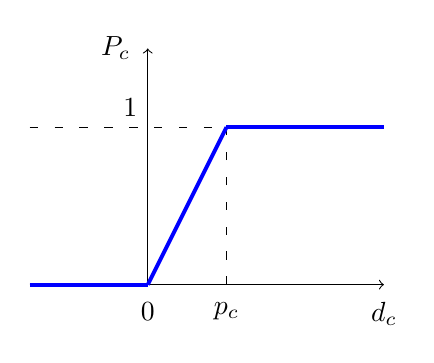
\begin{tikzpicture}
    % axes
    \draw[->] (-1.5,0) -- (3,0);
    \draw (3,0) node[below=0.1cm] {$d_c$};
    \draw [->] (0,0) -- (0,3);
    \draw (0,3) node[left=0.1cm] {$P_c$};
    \draw (0,0) node[below=0.1cm] {$0$};
    % dotted line for 1
    \draw[loosely dashed] (-1.5,2) -- (3,2);
    \draw (0,2) node[above left=0.01cm] {$1$};
    % negatif domain
    \draw[domain=-1.5:0,smooth,variable=\x,blue,line width=0.5mm] plot ({\x}, {0});
    % domain of growth
    \draw (1,0) node[below=0.1cm] {$p_c$};
    \draw[loosely dashed] (1,0) -- (1,2);
    \draw[domain=0:1,smooth,variable=\x,blue,line width=0.5mm] plot ({\x}, {2*(\x)});
    % strict préférence domain
    \draw[domain=1:3,smooth,variable=\x,blue,line width=0.5mm] plot ({\x}, {2});
    \end{tikzpicture}
    \end{center}
\end{minipage}%
\begin{minipage}{.5\textwidth}
    \begin{equation}
        P_c = \left\{
            \begin{array}{l c c}
                0               & \text{if}  & d_{c} \le 0 \\
                \frac{d_c}{p_c} & \text{if}  & 0 < d_c  < p_c \\
                1               & \text{if}  & d_{c} \ge p_c \\
            \end{array}
            \right .
            \label{eq:type3_criterion}
    \end{equation}
\end{minipage}
\caption{Preference function for criterion with linear preferences}
\end{figure}
The preference function for a criterion with linear preferences increases continuously with the difference of the evaluations between $0$ and some threshold $p_c$. If the difference is higher than this threshold, then the alternative with the highest evaluation is strictly prefered over the other.

This preference function is the first one that allows the decision maker to express valued preferences. If the difference of the evaluation lies between $0$ and $p_c$ the preference degree will be between $[0,1]$.

\subsubsection{Type 4: the level-criterion}
\begin{figure}[H]
\begin{minipage}{.5\textwidth}
    \begin{center}
    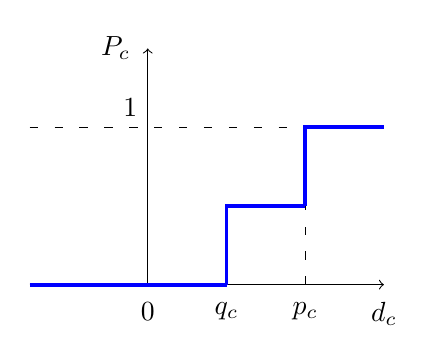
\begin{tikzpicture}
    % axes
    \draw[->] (-1.5,0) -- (3,0);
    \draw (3,0) node[below=0.1cm] {$d_c$};
    \draw [->] (0,0) -- (0,3);
    \draw (0,3) node[left=0.1cm] {$P_c$};
    \draw (0,0) node[below=0.1cm] {$0$};
    % dotted line for 1
    \draw[loosely dashed] (-1.5,2) -- (3,2);
    \draw (0,2) node[above left=0.01cm] {$1$};
    % negatif domain
    \draw[domain=-1.5:1,smooth,variable=\x,blue,line width=0.5mm] plot ({\x}, {0});
    % domain of growth
    \draw (2,0) node[below=0.1cm] {$p_c$};
    \draw[loosely dashed] (2,0) -- (2,2);
    \draw[domain=1:2,smooth,variable=\x,blue,line width=0.5mm] plot ({\x}, {1});
    \draw (1,0) node[below=0.1cm] {$q_c$};
    \draw[domain=0:1.025,smooth,variable=\y,blue,line width=0.5mm] plot ({1}, {\y});
    \draw[domain=1:2.025,smooth,variable=\y,blue,line width=0.5mm] plot ({2}, {\y});
    % strict preferenc domain
    \draw[domain=2:3,smooth,variable=\x,blue,line width=0.5mm] plot ({\x}, {2});
    \end{tikzpicture}
    \end{center}
\end{minipage}%
\begin{minipage}{.5\textwidth}
    \begin{equation}
        P_c = \left\{
            \begin{array}{l c c}
                0 & \text{if}  & d_{c} \le 0 \\
                \frac{1}{2} & \text{if}  & q_c < d_c   \le p_c \\
                1 & \text{if}  &  p_c < d_{c} \\
            \end{array}
            \right .
            \label{eq:type4_criterion}
    \end{equation}
\end{minipage}
\caption{Preference function for level-criterion}
\end{figure}

This criterion uses two parameters, the indifference threshold $q_c$ and the preference threshold $p_c$. If the difference of evaluations lies between these two thresholds, then the preference functions is equal to $0.5$.
This kind of function can be useful for criterions whose evaluations have discrete values (for example a criterion whose values can be ``green'', ``red'', ``blue'').
If the criterion's evaluations can take more than three values, an intuitive generalisation of this preference function with more than three levels can be used.

\subsubsection{Type 5: the criterion with linear preferences and indifference zone} \label{ss:pref_type_5}
\begin{figure}[H]
\begin{minipage}{.4\textwidth}
    \begin{center}
    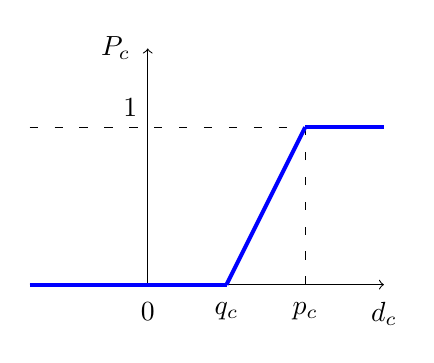
\begin{tikzpicture}
    % axes
    \draw[->] (-1.5,0) -- (3,0);
    \draw (3,0) node[below=0.1cm] {$d_c$};
    \draw [->] (0,0) -- (0,3);
    \draw (0,3) node[left=0.1cm] {$P_c$};
    \draw (0,0) node[below=0.1cm] {$0$};
    % doted line for 1
    \draw[loosely dashed] (-1.5,2) -- (3,2);
    \draw (0,2) node[above left=0.01cm] {$1$};
    % negatif domain
    \draw[domain=-1.5:1,smooth,variable=\x,blue,line width=0.5mm] plot ({\x}, {0});
    % domain of growth
    \draw (2,0) node[below=0.1cm] {$p_c$};
    \draw (1,0) node[below=0.1cm] {$q_c$};
    \draw[loosely dashed] (2,0) -- (2,2);
    \draw[domain=0:1,smooth,variable=\x,blue,line width=0.5mm] plot ({\x+1}, {2*(\x)});
    % strict preferenc domain
    \draw[domain=2:3,smooth,variable=\x,blue,line width=0.5mm] plot ({\x}, {2});
    \end{tikzpicture}
    \end{center}
\end{minipage}%
\begin{minipage}{.6\textwidth}
    \begin{equation}
        P_c = \left\{
            \begin{array}{l l c}
                0                       & \text{if}  & d_{c} \le q_c \\
                \frac{d_c-q_c}{p_c-q_c} & \text{if}  & q_c < d_c  \le p_c \\
                1                       & \text{if}  & p_c < d_c \\
            \end{array}
            \right .
            \label{eq:type5_criterion}
    \end{equation}
\end{minipage}
\caption{ Preference function for the criterion with linear and indifference zone}
\end{figure}

This preference function is a more general version of the Type 3 preference function. Here a parameter $q_c$ can be used to define an indifference threshold.

\subsubsection{Type 6: the gaussian criterion}
\begin{figure}[H]
\begin{minipage}{.4\textwidth}
    \begin{center}
    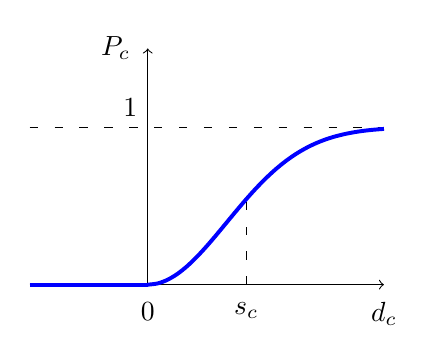
\begin{tikzpicture}
    % axes
    \draw[->] (-1.5,0) -- (3,0);
    \draw (3,0) node[below=0.1cm] {$d_c$};
    \draw [->] (0,0) -- (0,3);
    \draw (0,3) node[left=0.1cm] {$P_c$};
    \draw (0,0) node[below=0.1cm] {$0$};
    % doted line for 1
    \draw[loosely dashed] (-1.5,2) -- (3,2);
    \draw (0,2) node[above left=0.01cm] {$1$};
    % negatif domain
    \draw[domain=-1.5:0,smooth,variable=\x,blue,line width=0.5mm] plot ({\x}, {0});
    % domain of growth
    \draw (1.25,0) node[below=0.1cm] {$s_c$};
    \draw[loosely dashed] (1.25,0) -- (1.25,1.25);
    \draw[domain=0:3,smooth,variable=\x,blue,line width=0.5mm] plot ({\x}, {2-2*exp(-\x*\x/(2)});
    % strict preferenc domain
    %\draw[domain=2:3,smooth,variable=\x,blue,line width=0.5mm] plot ({\x}, {2});
    \end{tikzpicture}
    \end{center}
\end{minipage}%
\begin{minipage}{.6\textwidth}
    \begin{equation}
        P_c = \left\{
            \begin{array}{l l c}
                0                            & \text{if}  & d_{c} \le 0 \\
                1-e^{-d_c^2/2s_c^2} & \text{if}  & 0 < d_c  \\
            \end{array}
            \right .
            \label{eq:type6_criterion}
    \end{equation}
\end{minipage}
\caption{ Preference function for the gaussian criterion}
\end{figure}

This preference function leads to a preference increasing continuously with $d_c$. No threshold parameter is needed for this function but instead, the parameter $s_c$ must be fixed. This parameter indicates the difference $d_c$ needed to have a mean preference (0.39) of the criterion with the highest evaluation over the other.
The advantage of this preference function is that it will never reach 1. There is therefore no threshold of strict preference.


It is important to note that at most two parameters ($q_c$, $p_c$ or $s_c$) must be defined by the decision maker. As each of these parameters have a meaning in the real world, their assignation by the decision maker should not be an insurmountable task \cite{Brans2016}. \\
The choice of these parameters and of the preference functions consists in all the information \textit{within a criterion} \cite{Brans2016} that must be given by the decision maker.
This choice should be done with care as these parameters can have a crucial impact on the final ranking.
For example, choosing indifference thresholds too high for a specific criterion will have as consequence that this criterion will not have much impact as two alternatives will generally be equally preferred regarding to this criterion.
On the other hand, choosing a preference threshold too low will impoverish the preference structure, as alternatives will generally be strictly preferred the ones over the others, and the situation will be similar as when the preference was computed only by taking into account the sign of $d_c$.

\section{Enrichment of the dominance relationship} \label{sec:enrichment_dominance_relation}
\subsection { Global preference index} \label{subsec:global_pref_index}

After having computed the preference degrees for a given pair of alternatives for each criterion, a set of weights $w_c$ must still be defined in order to be able to compute the global preference index $\pi(a_i,a_j)$ of the alternative $a_i$ over the alternative $a_j$.
These weights $w_c$ represent the relative importance of a criterion $c$ compared to the others. The global preference index is given by:

\begin{equation}
    \pi(a_i,a_j) = \sum\limits^k_{c=1} P_c(a_i,a_j)\cdot w_c
    \label{eq:global_preference_index}
\end{equation}

The choice of the different $w_c$ consists in the information \textit{between criteria} \cite{Brans2016} that must be given by the decision maker.
Similarly as for the parameters giving information within a criterion, the choice of the $w_c$ is of the highest importance. For example, a criterion with a weight equal to zero would simply have no influence on the global preference index.

These weights factors must be positive as criteria would have a negative influence otherwise:

\begin{equation}
    w_c \ge 0 \qquad \forall c
    \label{eqn:wc_positif}
\end{equation}

As these parameters only consists of multiplicative constants, there is no inconvenient to choose them normalised:

\begin{equation}
    \sum\limits^k_{c=1} w_c = 1
    \label{eq:normalised_wc}
\end{equation}

Some relations can be deduced from the equations \eqref{eq:generalised_criterion} and \eqref{eq:global_preference_index}:

\begin{equation}
    \pi(a_i,a_i)=0
    \label{eq:pi_self}
\end{equation}
which states that an alternative is not preferred over itself, and
\begin{equation}
    0 \le \pi(a_i, a_j) \le 1
    \label{eq:pi_bounds}
\end{equation}
which holds since the weights are normalised and the $P_c$ are lower or equal to 1.
Furthermore, if $\pi(a_i, a_j)$ is strictly positive, then $\pi(a_j, a_i)$ will be equal to $0$, leading to:
\begin{equation}
    \pi(a_i, a_j) + \pi(a_j, a_i) \le 1
\end{equation}

It should also be clear that \cite{Brans2016}:
\begin{equation}
    \left \{
        \begin{array}[]{l c r}
            \pi(a_i,a_j) \approx 0 & \Leftrightarrow & \text{weak preference of $a_i$ over $a_j$} \\
            \pi(a_i,a_j) \approx 1 & \Leftrightarrow & \text{strong preference of $a_i$ over $a_j$}
        \end{array}
        \right .
    \label{eq:pi_0_1}
\end{equation}

All the pairwise preference indices $\pi(a_i, a_j)$ can be seen as forming an $n \times n$ preference matrix $\Pi$.

\subsection{Outranking flow} \label{sec:outranking_flow}

As just seen here above, $\pi(a_i,a_j)$ gives an indication of how $a_i$ is dominating $a_j$ on all the criterions.
This information is only related to a pair of alternatives and does not give a sufficient indication of the dominance of $a_i$ in the set $A$.

Such as for the \textsc{electre i} method (section \ref{sec:electre}), an outranking graph can be built. However, it will not be a binary outranking graph with arcs going from outranking alternatives to outranked alternatives anymore.
The graph will be a complete digraph on $n$ vertices representing the $n$ possible alternatives. The valued arc going from an alternative $a_i$ to an alternative $a_j$ will be valued $\pi(a_i,a_j)$ \cite{BransVincke85}.
This graph is therefore not a graph directly leading to an ordering, but will, for each pair of alternatives $a_i$ and $a_j$, give a quantified information of how much $a_i$ outranks $a_j$ and vice-versa.

This graph can be used to compute an \textit{outgoing outranking flow} and an \textit{incoming outranking flow} for each alternative \cite{Bertrand2002}. \\
The outgoing flow is given by:
\begin{equation}
    \phi^+(a_i) = \frac{1}{n-1}\sum\limits^n_{j=1} \pi(a_i,a_j)
    \label{eq:outgoing_flow}
\end{equation}
This flow indicates how much alternative $a_i$ is dominating or outranking on average the remaining $n-1$ alternatives. The higher this flow, the more $a_i$ should be preferred by the decision maker.

Similarly, the incoming flow is defined by \cite{Bertrand2002}:
\begin{equation}
    \phi^{-}(a_i) = \frac{1}{n-1}\sum\limits^n_{j=1} \pi(a_j,a_i)
    \label{eq:incoming_flow}
\end{equation}
This flow indicates how much alternative $a_i$ is outranked on average by the $n-1$ other alternatives. The lower this flow, the more alternative $a_i$ should be preferred.

One can see in the expressions of the outranking flows that the summations of the preference index are divided by $n-1$. This is done to ensure that the outranking flows will be lower or equal to $1$ (the summations consist of sums on $n$ terms lower than $1$ from which at least one is null by \eqref{eq:pi_self}).

The netflow score can be obtained by subtracting the incoming flow from the outgoing flow:

\begin{equation}
    \phi(a_i) = \phi^+(a_i) - \phi^-(a_i)
    \label{eq:netflow}
\end{equation}

\section{Decision aid}
\subsection{\textsc{Promethee i}}
To help the decision maker in his task, the \textsc{promethee} methods will rank the alternatives according to their outranking flows.

The two complete preorders ($P^+$,$I^+$) and ($P^-$,$I^-$) obtained with the outranking flows are defined as follow \cite{Bertrand2002}:

\begin{equation}
    \forall a_i, a_j \in A \left \{
        \begin{array}[]{l c c}
            a_iP^+a_j & \Leftrightarrow & \phi^+(a_i) > \phi^+(a_j) \\
            a_iI^+a_j & \Leftrightarrow & \phi^+(a_i) = \phi^+(a_j)
        \end{array}
        \right .
    \label{eq:P1_positif_ranking}
\end{equation}
\begin{equation}
    \forall a_i, a_j \in A \left \{
        \begin{array}[]{l c c}
            a_iP^-a_j & \Leftrightarrow & \phi^-(a_i) < \phi^-(a_j) \\
            a_iI^-a_j & \Leftrightarrow & \phi^-(a_i) = \phi^-(a_j)
        \end{array}
        \right .
    \label{eq:P1_negatif_ranking}
\end{equation}

The \textsc{promethee i} ranking is made by taking the intersection of these two preorders. An alternative $a_i$ is preferred over another alternative $a_j$ according to \mbox{\textsc{promethee i}} if both its outgoing flow and its incoming flow are better (respectively greater and smaller) than the ones of $a_j$. If both the flows are equal for the two alternatives, then the alternatives will be indifferent, and if none of these two cases hold, then the alternatives will be said to be incomparable \cite{Bertrand2002}:


\begin{equation}
  \forall a_i, a_j \in A: \left\{
    \renewcommand{\arraystretch}{1.75}
    \begin{array}{l l}
      a_iPa_j  & \Leftrightarrow \ \ \left\{
          \begin{array}{l }
              a_iP^+a_j \text{ and } a_iP^-a_j \\
              a_iP^+a_j \text{ and } a_iI^-a_j \\
              a_iI^+a_j \text{ and } a_iP^-a_j \\
          \end{array} \right . \\
      a_iIa_j & \Leftrightarrow \qquad a_iI^+a_j \text{ and } a_iI^-a_j \\
      a_iRa_j & \Leftrightarrow \qquad \text{else} \\
    \end{array} \right . \\
    \label{eq:PI_ranking}
\end{equation}



\subsection{\textsc{Promethee ii}} \label{sec:decision_aid_pii}

It can happen that the decision maker wishes to obtain a complete ordering of the alternatives (without any incomparabilities). This can be done using \textsc{promethee ii}. This method builds a ranking based on the net flow score of each alternatives:

\begin{equation}
    \forall a_i,a_j \in A \left \{
        \begin{array}[]{l}
            a_iPa_j \Leftrightarrow \phi(a_i) > \phi(a_j) \\
            a_iIa_j \Leftrightarrow \phi(a_i) = \phi(a_j) \\
        \end{array}
        \right .
    \label{eq:PII_ranking}
\end{equation}

As it can be seen, using \textsc{promethee ii}, two alternatives can be either prefered the one over the other ($P$) either indifferent ($I$). Two alternatives can therefore not be incomparable, leading to a complete preorder of the alternatives.

Furthermore, it should be pointed out that the outgoing, incoming or net flows are not just some artificial and arbitrary constructions made to aggregate the pairwise preferences.
In fact, it can be shown that the net flow score is the centered score that minimizes the sum of the square deviations for the pairwise preferences of the alternatives \cite{mareschal2008rank}.

In other words, if $Q$ is the sum of the square deviations between a centered score $s$ and the pairwise preferences, with $s_i$ being the score of the alternative $a_i$:

\begin{equation}
    Q = \sum\limits_{i=1}^n\sum\limits_{j=1}^n\big[(s_i-s_j) - (\pi(a_i, a_j) - \pi(a_j,a_i))\big]^2
    \label{eqn:square_deviations_sum}
\end{equation}

then $Q$ will be minimal when the score $s_i$ of alternatives are proportionals to their net flows:

\begin{equation}
    s_i = \frac{1}{n}\sum\limits_{j=1}^n (\pi(a_i,a_j)-\pi(a_j,a_i)) = \frac{n-1}{n} \phi(a_i)
    \label{eqn:score_prop_netflow}
\end{equation}

\subsection{Conclusion}

There exist other variations of \textsc{promethee} than the \textsc{promethee i} and \textsc{promethee ii} methods but these will not be detailed here and the interested reader can refer to \cite{Brans2016} for additional information.

There also exists an additional tool, named \textsc{gaia} (Geometrical Analysis for Interactive Assistance), which is, as its name suggests, a tool aimed at performing an interactive visualisation of the data.
Once again, this method will not be detailed here and the interested reader can refer to \cite{Brans2016} or \cite{Bertrand2002} for additional information.

Finally, it should also be noted that part the success of \textsc{promethee} is due to the existence of userfriendly software (such as \textit{D-Sight}) that helps the decision maker in the visualisation of the alternatives and the influence of the different parameters of the method \cite{DeSmet2013}.

A criticism that is often addressed to the \textsc{promethee} methods is that it is subject to the \textit{rank reversal} phenomenon. An introduction to this phenomenon will be presented in the next chapter. Then, two variations of \textsc{promethee ii} which are aimed at reducing these rank reversals will be studied.

